\documentclass{rapport}
\usepackage[utf8]{inputenc}

\usepackage{pifont} % Pour les symboles appelés par la macro \ding
\usepackage{url} % Comme son nom l'indique, pour les url...

\usetikzlibrary{positioning} % Bibliothèque tikz pour positionner des nœuds relativement à d'autres

\usepackage[colorlinks, citecolor=red!60!green, linkcolor=blue!60!green, urlcolor=magenta]{hyperref} % Pour que les liens soient cliquables. Les options permettent de mettre les liens en couleur.

\usepackage{algorithm}
\usepackage{algo}
\usepackage{colorationSyntaxique}
\usepackage{listings}
\usepackage{xcolor}



% Pour un rapport en français 
\usepackage[francais]{babel} % Commenter pour un rapport en anglais
\renewcommand\bibsection{\section*{Bibliographie}} % Commenter pour un rapport en anglais

% \englishTitlePage % Décommenter pour une page de titre en anglais


\pagestyle{fancy}
\renewcommand{\sectionmark}[1]{\markboth{\thesection.\ #1}{}}
\fancyfoot{}

\fancyhead[LE]{\textsl{\leftmark}}
\fancyhead[RE, LO]{\textbf{\thepage}}
\fancyhead[RO]{\textsl{\rightmark}}

\def\Latex{\LaTeX\xspace}
\def\etc{\textit{etc.}\xspace}

\lstset{                  % Specify language
    basicstyle=\ttfamily\small,     % Code font and size
    keywordstyle=\color{blue},      % Color for keywords
    commentstyle=\color{gray},      % Color for comments
    stringstyle=\color{red},        % Color for strings
    numbers=left,                   % Add line numbers
    numberstyle=\tiny\color{gray},  % Style for line numbers
    % frame=single,                   % Add a border around code
    breaklines=true,                % Line wrapping
    % backgroundcolor=\color{gray!10} % Light gray background
}



\title{Placement des threads sur les cœurs: Threads affinity}
\author{Francois Flandin}
\supervisor{Pr Sid Touati}
\date{Premier semestre de l'annee 2024-2025}

% \universityname{Université Côte d'Azur} % Nom de l'université.
\type{TP} % Type de document
% \formation{Master Informatique} % Nom de la formation

% Retrouver les autres options possibles dans le document rapport.pdf

\begin{document}

\maketitle

\clearpage
\tableofcontents

\clearpage


\section{Introduction}
Ce rapport s'inscrit dans le cadre des travaux pratiques visant à explorer les performances des programmes parallèles en étudiant l'impact du placement des threads sur les cœurs du processeur. L'objectif principal est de mesurer les variations de performances en fonction des différents paramètres d'exécution et de compiler des benchmarks pour analyser la stabilité des résultats.
\newline
Pour cela, un code de multiplication de matrices massivement parallèle, implémenté avec OpenMP, a été utilisé comme point de départ. Différentes configurations ont été testées, en variant les stratégies de placement des threads sur les cœurs logiques. Les résultats obtenus ont été analysés à l'aide de techniques statistiques et de visualisations graphiques dans l'environnement R, afin de mettre en évidence les comportements de performance dans des contextes d'exécution variés.
\newline
Ce document présente dans un premier temps la méthodologie employée, suivie d'une analyse des résultats expérimentaux, et conclut par une discussion sur les implications des choix de placement des threads sur l'efficacité des calculs parallèles.

\section*{Environnement Expérimental}
    \subsection*{Micro-Architecture}
    Dans cette partie sera detaillée la micro-architecture de la machine de tests.
    \newline\newline
    \textbf{Nom de modèle :} 11th Gen Intel(R) Core(TM) i5-1135G7 @ 2.40GHz
    \newline
    \textbf{Taille des adresses :} 39 bits physical, 48 bits virtual
    \newline
    \textbf{Coeurs physiques :} 4
    \newline
    \textbf{Taille de ligne de cache :} 64 octets

    \begin{table}[H]
        \centering
        \begin{tabular}{|l|c|c|c|c|}
            \hline
            \multicolumn{5}{|c|}{Graphical Topology} \\
            \hline
            Coeurs & \enspace0\enspace\enspace4 &\enspace1\enspace\enspace5 &\enspace2\enspace\enspace6 &\enspace3\enspace\enspace7 \\
            \hline
            Cache L1 & \enspace48 kB &\enspace48 kB &\enspace48 kB &\enspace48 kB \\
            \hline
            Cache L2 & 1MB & 1MB & 1MB & 1MB \\
            \hline
            Cache L3 & \multicolumn{4}{|c|}{8 MB} \\
            \hline
        \end{tabular}
        \caption{Topologie de la machine de tests}
        \label{tab:graph_characteristics}
    \end{table}
    
    
    \subsection*{Environnement Logiciel}
    Dans cette partie sera détaillée la partie logiciel de la machine de test, les fichiers scripts pour changer entre machine allégée et machine classique sont fournis dans l'archive.
    \newline\newline
    \textbf{Distribution :} Fedora Linux v40 WorkStation
    \newline
    \textbf{Compilateur utilisé :} \texttt{gcc} version 14.2.1 20240912 avec option \texttt{-O2}
    \newline
    \textbf{Outil de mesure des temps d'exécution :} Commande \texttt{/bin/time}.

    \section*{Configuration expérimentale}
    \subsection*{Processus en activité}
    \begin{verbatim}
    > ps -x
    PID TTY      STAT   TIME COMMAND
   1263 ?        Ss     0:00 /usr/lib/systemd/systemd --user
   1265 ?        S      0:00 (sd-pam)
   1284 tty1     Ss     0:00 -zsh
   1898 tty1     R+     0:00 ps -x
    \end{verbatim}
    \subsubsection*{Description des processus}
    Voici ce que font les processus en cours d'exécution.
    \newline\newline
    \textbf{systemd :} C'est un système d'initialisation et de gestion de services sous Linux, conçu pour démarrer, arrêter et superviser les processus, tout en offrant une gestion centralisée des sessions et des ressources.
    \newline
    \textbf{sd-pam :} \textit{systemd-PAM} C'est un utilitaire de \texttt{systemd} pour gérer les sessions.
    \newline
    \textbf{zsh :} C'est le shell qui est lancé pour exécuter les commandes.
    \newline
    \textbf{ps -x :} C'est la commande qui a été lancée pour voir les processus.
    
    \subsection*{Méthodologie de récolte des données expérimentales}
    
    Plusieurs scripts ont été réalisés afin de compiler le programme source sous différentes versions pour les besoins du TP, mais aussi afin de réaliser les différents benchmarks.
    \newline Pour mesurer le temps d'exécution, on utilisera la commande \texttt{/bin/time} sur 50 exécutions consécutives, ces données seront ensuite analysées à l'aide d'un programme \texttt{R}.

\section{Compiler le code C, les differences entre \texttt{gcc} et \texttt{icx}}
Dans cette partie, seront presentées les différences de librairies utilisées entre \texttt{gcc} et \texttt{icx}:
\subsection*{Librairies \texttt{matrix-icx}}
\begin{lstlisting}
> ldd matrix-icx

linux-vdso.so.1 (0x00007fca6e109000)
libm.so.6 => /lib64/libm.so.6 (0x00007fca6e004000)
libiomp5.so => /opt/intel/oneapi/2025.0/lib/libiomp5.so (0x00007fca6dc00000)
libc.so.6 => /lib64/libc.so.6 (0x00007fca6da0f000)
/lib64/ld-linux-x86-64.so.2 (0x00007fca6e10b000)
librt.so.1 => /lib64/librt.so.1 (0x00007fca6dfff000)
libdl.so.2 => /lib64/libdl.so.2 (0x00007fca6dffa000)
libpthread.so.0 => /lib64/libpthread.so.0 (0x00007fca6da0a000)
\end{lstlisting}
\subsection*{Librairies \texttt{matrix-gcc}}
\begin{lstlisting}
> ldd matrix-gcc

linux-vdso.so.1 (0x00007fb525b31000)
libgomp.so.1 => /lib64/libgomp.so.1 (0x00007fb525aba000)
libc.so.6 => /lib64/libc.so.6 (0x00007fb5258c9000)
/lib64/ld-linux-x86-64.so.2 (0x00007fb525b33000)
\end{lstlisting}

\subsection*{Comparaison}
On remarque que \texttt{icc} utilise bien plus de librairies que \texttt{gcc}, avec l'utilisation des librairies \texttt{libpthread}, \texttt{libdl} ou encore \texttt{librt}.
\newline Cependant la plus grande différence est la librairie \texttt{OpenMP} qu'ils utilisent, à savoir \texttt{libiomp5} pour \texttt{icc} et \texttt{libgomp} pour \texttt{gcc}.


\section{Stabilité des performances d'un programme}
\subsection{Résultat de \texttt{summary()} en R}
\subsubsection*{matrix-gcc}
\begin{lstlisting}
> summary(X)
Min. 1st Qu.  Median    Mean 3rd Qu.    Max.
2.300   2.410   2.465   2.489   2.547   3.100
\end{lstlisting}
\subsubsection*{matrix-icx}
\begin{lstlisting}
> summary(Y)
Min. 1st Qu.  Median    Mean 3rd Qu.    Max.
5.420   5.643   5.770   5.828   5.987   6.720
\end{lstlisting}
On remarque que, d'une part \texttt{gcc} propose de meilleures performances que \texttt{icx} avec \texttt{OpenMP}, et d'autre part, que \texttt{gcc} propose des temps plus stables que \texttt{icx}, avec un écart-type de 0.8 secondes pour \texttt{gcc}, tandis que l'écart-type pour \texttt{icx} est de 1.3 secondes.


\subsection{Boxplots}

\begin{figure}[H]
    \centering
    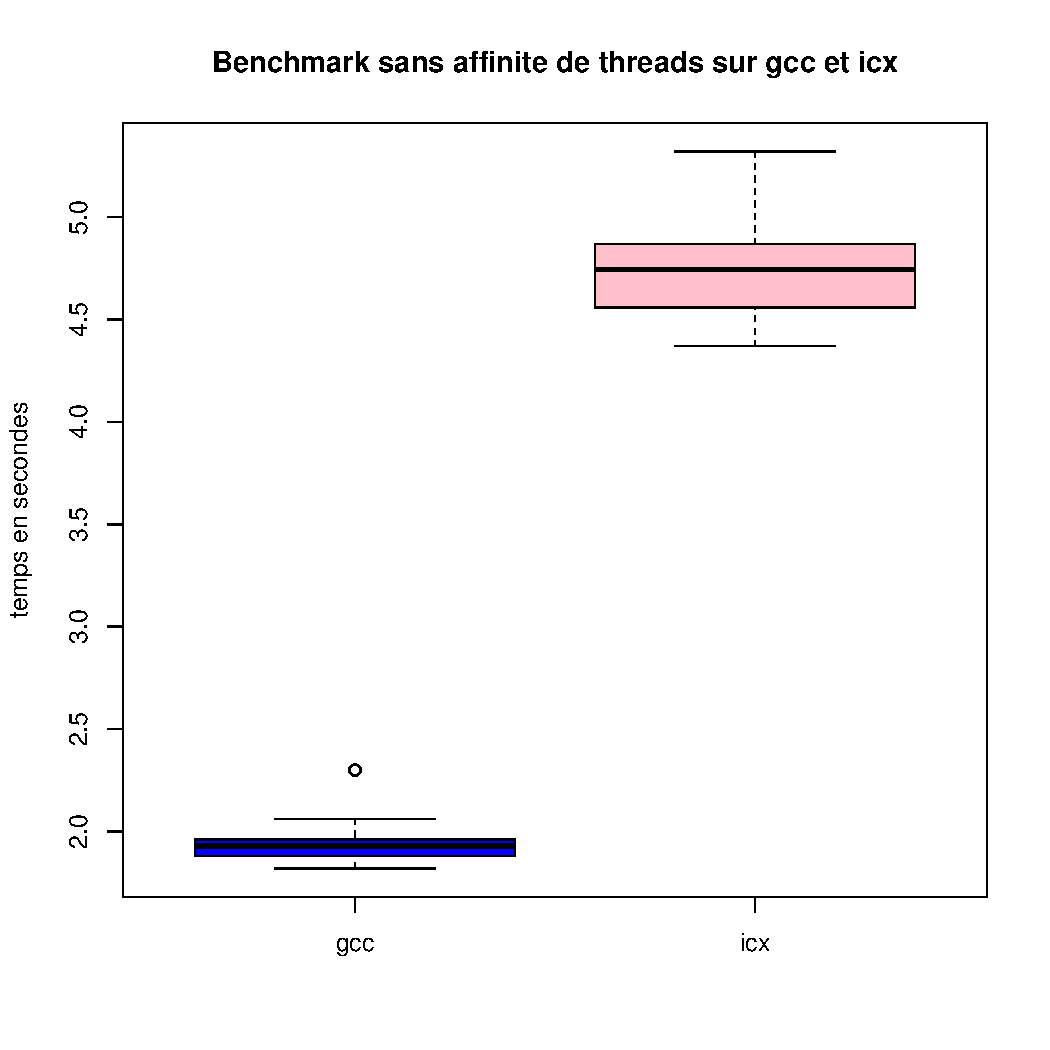
\includegraphics[width=1\textwidth]{../tp3/benchmark/bench_no_affinity.pdf}
    \caption{Boxplots des temps d'exécution de matrix-gcc et matrix-icx.}
\end{figure}

\textbf{Analyse:} Ce graphe montre que \texttt{gcc} est plus efficace que \texttt{icx} sans affinité de threads.


\section{Analyse des stratégies \texttt{scatter} et \texttt{compact}}

\begin{figure}[H]
    \centering
    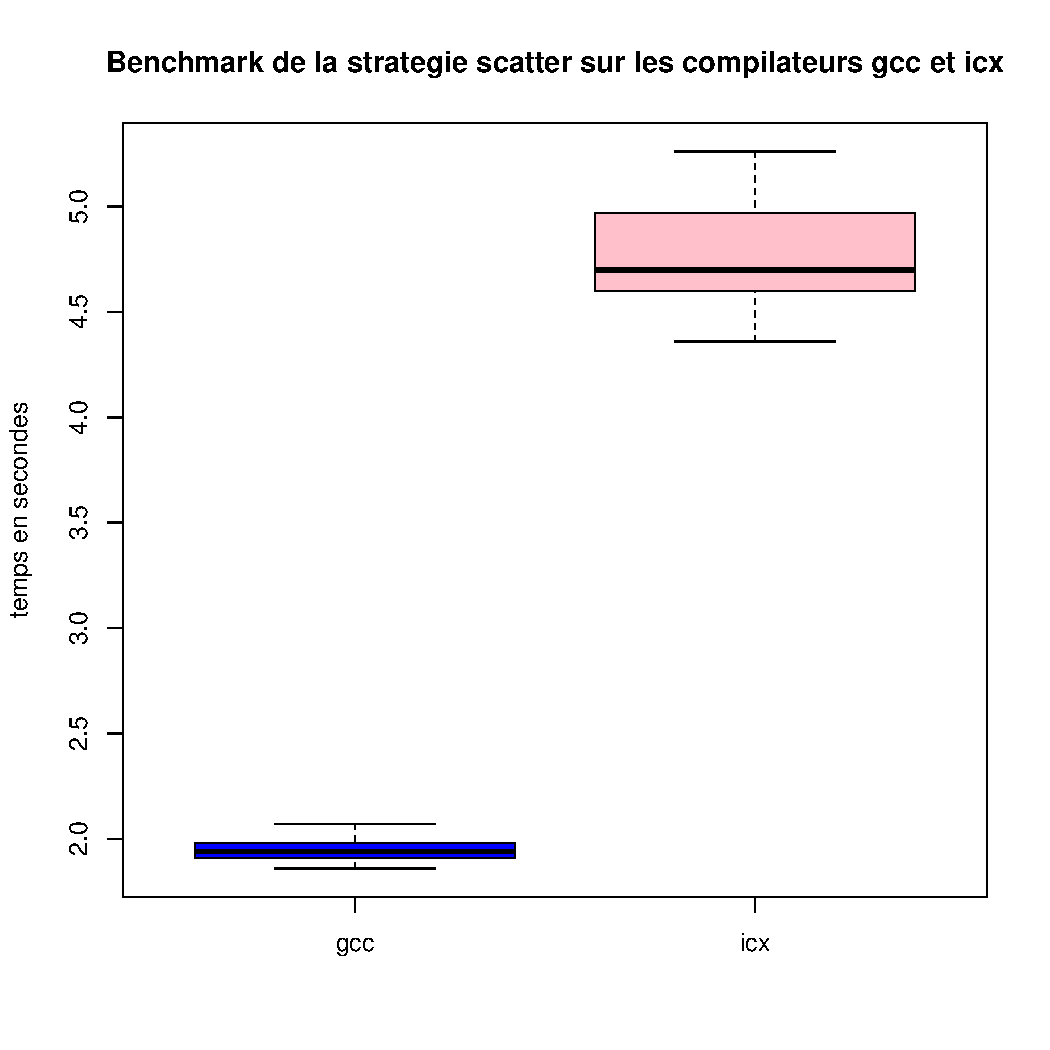
\includegraphics[width=1\textwidth]{../tp3/benchmark/benchmark_scatter.pdf}
    \caption{Boxplots des temps d'execution de matrix-gcc et matrix-gcc avec l'affinite de threads \texttt{scatter}.}
\end{figure}

\begin{figure}[H]
    \centering
    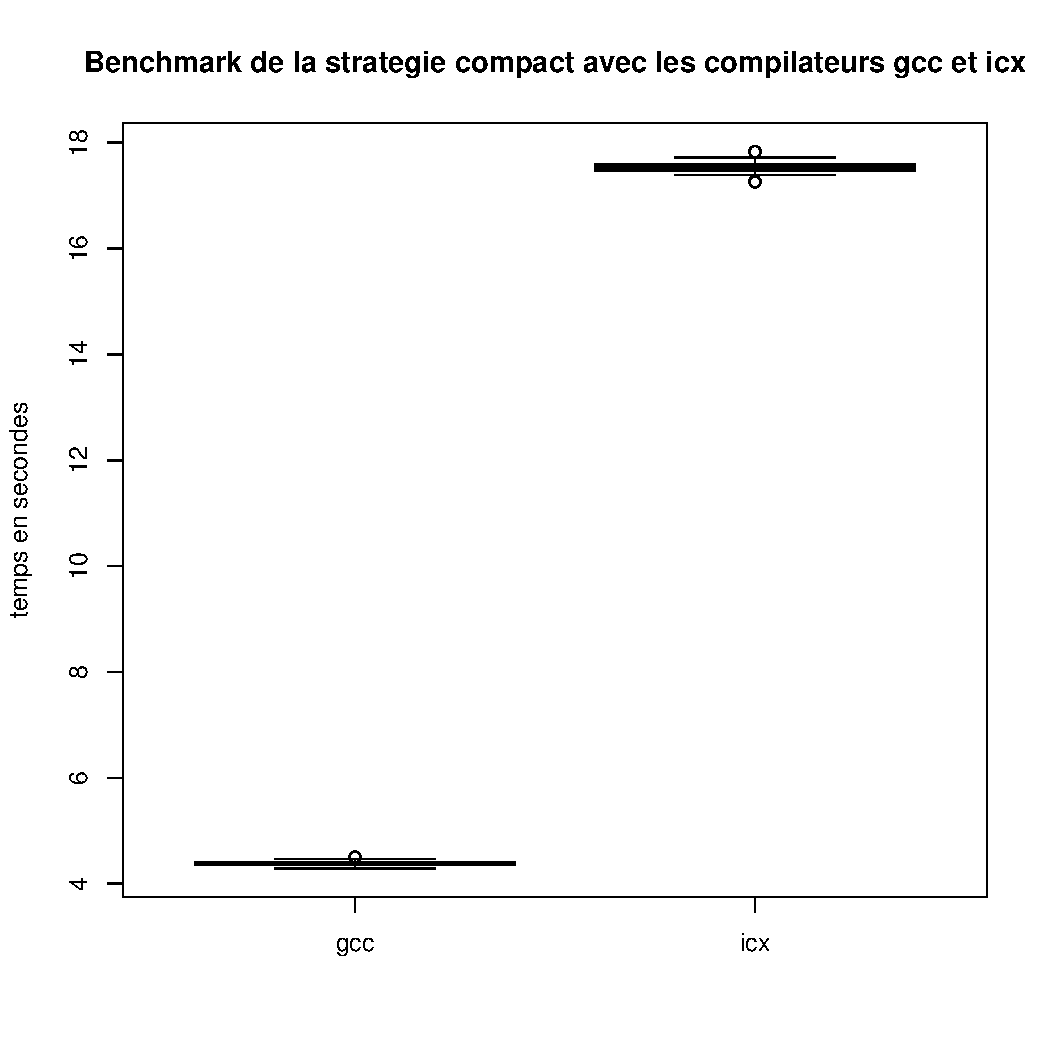
\includegraphics[width=1\textwidth]{../tp3/benchmark/benchmark_compact.pdf}
    \caption{Boxplots des temps d'execution de matrix-gcc et matrix-gcc avec l'affinite de threads \texttt{compact}.}
\end{figure}

\section{Conclusion}
Au cours de ces expériences, nous avons comparé la vitesse ainsi que la stabilité d'exécution de la libraire \texttt{OpenMP} avec \texttt{gcc} et \texttt{icx}, les résultats nous montrent que de manière générale, \texttt{gcc} produit des codes plus efficaces que \texttt{icx}. \newline De plus, des benchmarks sur d'autres stratégies d'affinité de thread ont été réalisés, montrant que la stratégie \texttt{scatter}, qui vise a séparer les threads sur lesquels on effectue l'exécution, est plus performante que la stratégie \texttt{compact}, qui elle vise a rapprocher les threads sur lesquel on effectue l'exécution. Cela peut être dû au fait que la stratégie \texttt{compact} utilise des coeurs logiques qui se trouvent sur le même coeur physique, ce qui pourrait diminuer l'efficacité par rapport à des threads sur des coeurs physiques séparés.

\end{document}
